\chapter{Results1}
\label{ch:Results1}
\textit{This chapter explores}

\startcontents[chapters]{\vspace{-1.4cm}}
\singlespacing
\printcontents[chapters]{}{1}{\section*{ }\setcounter{tocdepth}{1}}
\doublespacing

\section{Introduction}

\subsection{Difficulties in defining and diagnosing sepsis} \label{ssec:Sepsisdefinition}

Sepsis is currently defined as ``life-threatening organ dysfunction caused by a dysregulated host response to infection''. 

\subsection{Aims}

\begin{enumerate}
	\item Aim 1
	\item Aim 2
	\item Aim 3
\end{enumerate}

\section{Results: sepsis}

\subsection{Description of sepsis cohorts} \label{ssec:cohort_description}

\begin{figure}[htbp]
\centering
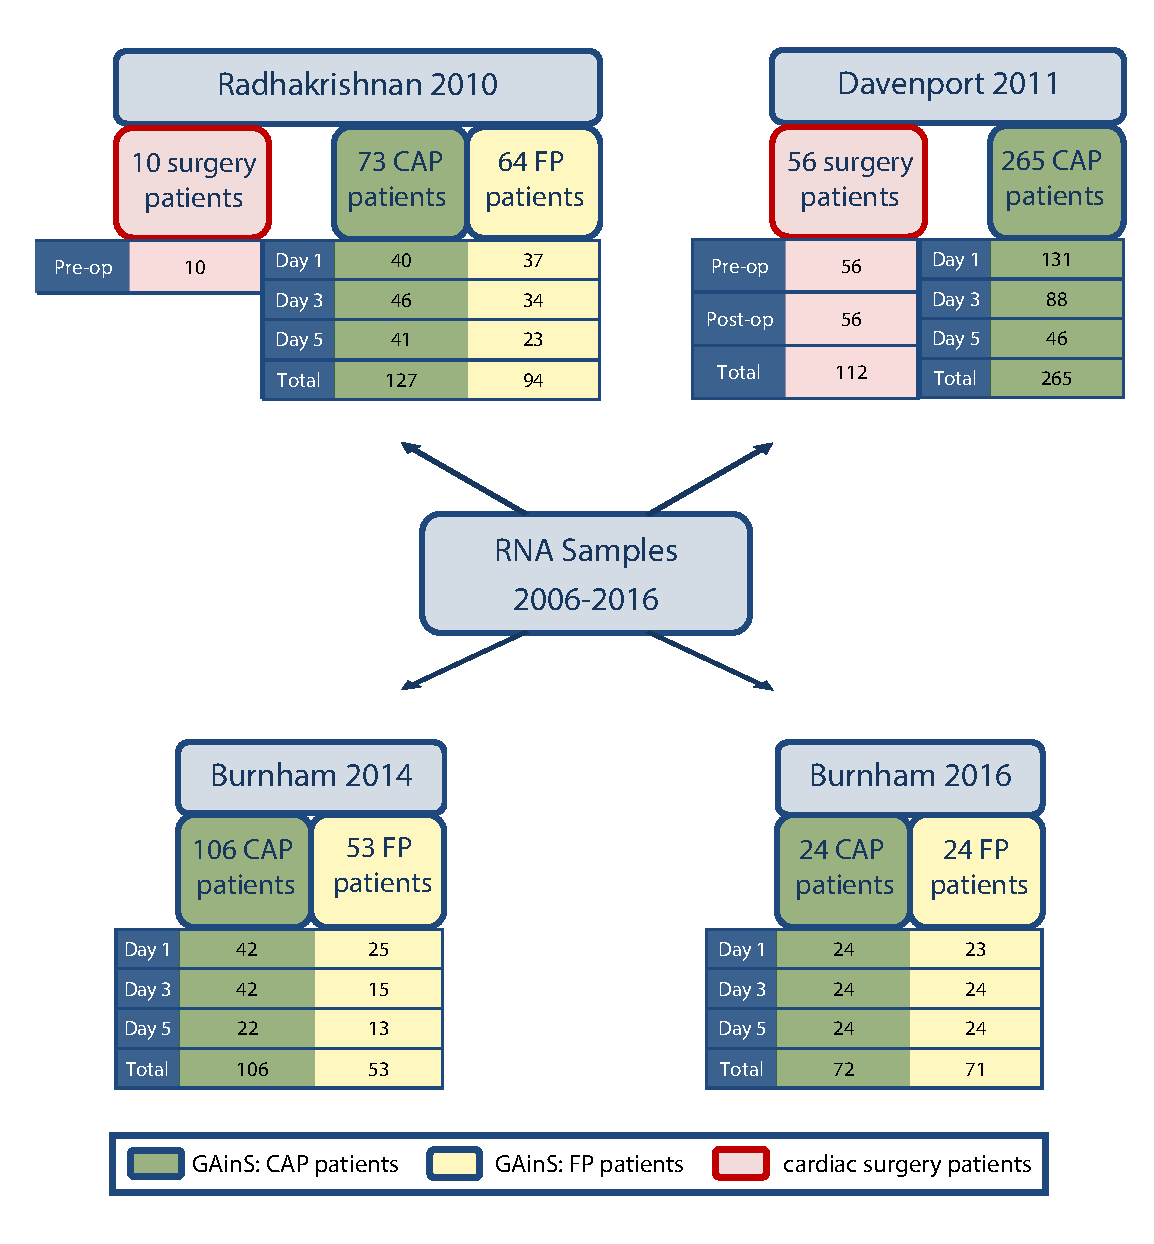
\includegraphics[width=\textwidth]{./Results1/CohortOverview}
\caption[Overview of GAinS gene expression cohorts]{\textbf{Overview of the GAinS gene expression datasets analysed in this thesis.} \\
The number of samples for which gene expression data are available following quality control is given for each of the four cohorts analysed in this thesis. This is subdivided according to the cause of sepsis (CAP (\emph{green}) or FP (\emph{yellow})), given the focus on source of infection in this chapter. Cohorts are named according to the person who generated the data and the year this was done. Samples from elective cardiac surgery patients (\emph{red}), taken before and after their operation by Eduardo Svoren, are also included in the Radhakrishnan 2010 and Davenport 2011 cohorts.}
\label{fig:CohortOverview}
\end{figure}

In this chapter, I analyse sepsis microarray gene expression data processed in several different batches over a six year period (Fig. \ref{fig:CohortOverview}). 

\section{Discussion}

\section{Conclusions}

The analysis presented in this chapter combines multiple transcriptomic datasets to compare the systemic inflammatory response across different sources. This demonstrates that a significant proportion of the sepsis transcriptomic response is shared between CAP and FP patients, although there is some specificity according to infection site. These findings may have implications for the management of sepsis, suggesting patient stratification and targeting treatment on the basis of cause of sepsis could be beneficial. In addition, future research and drug development may benefit from the use of more homogeneous cohorts. However, aspects of the transcriptomic response are shared across sepsis due to CAP and FP and sterile SIRS, indicating that findings in one SIRS subtype might be relevant to another and that similar treatment strategies could be considered. 